% ------------ LSA-proceedings-template.tex  -- LSA proceedings template ---------------------------------------------------------------------------
% created by Sarah E. Murray, 24 April 2017 based on the LSA's stylesheet
% http://journals.linguisticsociety.org/proceedings/index.php/PLSA/pages/view/instructions
%Updated by Patrick Farrell, February 1, 2019.
%
% ------------ begin preamble -----------------------------------------------------------------------------------------
 \documentclass[12pt,letterpaper]{article}	
% ------------ personal packages ----------------------------------------------------------------------------
\usepackage{linguex}	%http://texdoc.net/texmf-dist/doc/latex/linguex/linguex-doc.pdf
% ------------ LSA page layout and packages ----------------------------------------------------------------------------
\usepackage{times}
\usepackage{natbib}
 	\setcitestyle{semicolon,aysep={},yysep={,},notesep={; }}
\usepackage{lipsum}          % this and the following package and the settings beneath them are for maintaining indentation and still having ragged-right aligmnent
\usepackage{ragged2e}
\setlength\RaggedRightParindent{0.3in}
\RaggedRight

\usepackage{graphicx}
\usepackage{booktabs}
\usepackage{amssymb} % checkmark
\usepackage{qtree}
\qtreecenterfalse
\newcommand{\sem}[1]{\mbox{$[\![$#1$]\!]$}}
\newcommand{\lam}{$\lambda$}
\newcommand{\lan}{$\langle$}
\newcommand{\ran}{$\rangle$}
\newcommand{\type}[1]{\ensuremath{\left \langle #1 \right \rangle }}
\renewcommand{\firstrefdash}{}

\usepackage{fullpage} 
\usepackage[compact]{titlesec}
	\titleformat{\section}[runin]{\normalfont\bfseries}{\thesection.}{.5em}{}[.]
	\titleformat{\subsection}[runin]{\normalfont\scshape}{\thesubsection}{.5em}{}[.]
\usepackage[usenames,dvipsnames]{color}	
\usepackage[colorlinks,allcolors={black},urlcolor={blue}]{hyperref} 		%likes to be last package 
% -------------- personal definitions ---------------------------------------------------------------------------------------------------------   
% -------------- LSA definitions ---------------------------------------------------------------------------------------------------------           
\setlength\parindent{0.3in}			%paragraphs indented 0.3inches
\setlength\intextsep{6pt}			%spacing before and after tables
\setlength\abovecaptionskip{6pt}	%spacing between figure and caption
%-------------------------------------------------------------- format title --------------------------------------
\makeatletter
\def\@maketitle{%
  \newpage
  \begin{center}%
  \let \footnote \thanks
    {\normalfont\bfseries \@title \par}%
    {\vskip .5em%\vskip 6pt%
      \begin{tabular}[t]{c}%
        \@author
      \end{tabular}\par}%
  \end{center}%
  \par}
\makeatother
%-------------------------------------------------------------- format abstract environment --------------------------------------
% Abstracts have to be 12pt, indented 1.4 inches on each side, and inline with the label
\renewenvironment{abstract}{%
\noindent\begin{minipage}{1\textwidth}
\setlength{\leftskip}{0.4in}
\setlength{\rightskip}{0.4in}
\textbf{Abstract.}}
{\end{minipage}}
%-------------------------------------------------------------- format keywords environment --------------------------------------
% Abstracts have to be 12pt, indented 1.4 inches on each side, and inline with the 
\newenvironment{keywords}{%
\vspace{.5em}
\noindent\begin{minipage}{1\textwidth}
\setlength{\leftskip}{0.4in}
\setlength{\rightskip}{0.4in}
\textbf{Keywords.}}
{\end{minipage}}
%-------------------------------------------------------------- title information --------------------------------------%
\title{
	Adjective ordering in Tagalog:\\
	A cross-linguistic comparison of subjectivity-based preferences
} 
%
\author{Suttera Samonte \& Gregory Scontras\footnote{We gratefully acknowledge the support of the Linguistic Society of America's Committee on Ethnic Diversity in Linguistics, who awarded a travel grant to Suttera Samonte so that she could present this work at the annual meeting in New York. %
		Authors: Suttera Samonte, University of California, Irvine (\href{mailto:suttera.samonte@gmail.com}{suttera.samonte@gmail.com}),
		Gregory Scontras, University of California, Irvine (\href{mailto:g.scontras@uci.edu}{g.scontras@uci.edu}).}}
% ------------ end preamble ------------------------------------------------------------------------------------------------
% 
%
%
% ------------ begin main document --------------------------------------------------------------------------------------
 
 
\begin{document} 

%%If using linguex, need the following commands to get correct LSA style spacing
%% these have to be after  \begin{document}
\setlength{\Extopsep}{6pt}
\setlength{\Exlabelsep}{9pt}		%effect of 0.4in indent from left text edge
%%
 
\maketitle

\begin{abstract}
	Previous studies have shown that speakers have robust adjective ordering preferences. For example, in English, \emph{big red apple} is strongly preferred to \emph{red big apple}. Recently, \cite{scontrasetal2017adjectives}
	showed that an adjective's distance from the noun it modifies is best predicted by the adjective's subjectivity, with less subjective adjectives preferred closer to the modified noun. However, this finding was limited to English. The current study investigates the status of subjectivity-based adjective ordering preference in Tagalog, a language that forms its modification structures with the conjunction-like \textsc{linker} particle. Using Tagalog translations of the original English materials, we show that subjectivity predicts ordering preferences in Tagalog, as it does in English.
\end{abstract}

\begin{keywords}
	Tagalog; adjective ordering; \textsc{linker}; subjectivity
\end{keywords}

\section{Introduction}

Adjective ordering preferences determine the relative order of multi-adjective strings. When speakers form multi-adjective strings (e.g., \emph{big red apple}), these preferences ensure that the ordering of the adjectives is non-arbitrary.  Curiously, the very same preferences documented in English have been reported in a host of different languages, including Hungarian, Telugu, Mandarin Chinese, and Dutch \citep[e.g.,][]{Martin1969competence,hetzron1978,dixon1982,sproatshih1991}.  
Recently, \cite{scontrasetal2017adjectives} showed that adjective subjectivity is a robust predictor of ordering preferences in English: less subjective adjectives occur closer to the modified noun. The current study investigates the extent to which this pattern holds in a language with a diverging modification strategy. To that end, we examine ordering preferences in Tagalog. 

Unlike English, Tagalog adjectives require a linking particle (\emph{-ng}/\emph{na}) in order to participate in modification structures \citep{foley1975,rubin1994,kaufman2009}. Some authors analyze the semantic contribution of \textsc{linker} similarly to that of conjunction (\citealp{rubin1994},\\ \noindent\citealp{scontrasnicolae2014}). However, in English, conjunction has been claimed to neutralize adjective ordering preferences \citep{fordolson1975,byrne1979}. We therefore set out to determine (i) whether Tagalog possesses ordering preferences in the presence of \textsc{linker}, and, if so, (ii) to what extent adjective subjectivity predicts those preferences. The paper is structured as follows. In Section \ref{background}, we survey the empirical findings regarding subjectivity-based ordering preferences in English, then provide relevant background on modification structures in Tagalog. We then present the findings from two experiments. First, in Section \ref{expt1}, we document adjective ordering preferences in Tagalog. Next, in Section \ref{expt2}, we measure Tagalog adjective subjectivity. In Section \ref{comparison}, we compare the results of the two experiments in order to determine whether subjectivity predicts ordering preferences in Tagalog. Section \ref{discussion} concludes with a comparison of our Tagalog results and the English results from \cite{scontrasetal2017adjectives}.

% What sounds more natural: ``the small brown cardboard box'' or ``the cardboard brown small box''? Most speakers of English will agree that the former phrase sounds the most natural, and this result extends to speakers of many different languages such as Hungarian, Telugu, Mandarin Chinese, Dutch, etc. (Martin, 1969b; Hetzron, 1978; Dixon, 1982; Sproat and Shih, 1991; LaPolla and Huang, 2004). However, previous research was unable to conclude why humans form these specific ordering preferences, leaving open to question which factors best predict adjective ordering preferences. The current study looks to revisit these questions, as well as expand recent research to investigate whether adjective ordering preferences are present in languages that display unparallel adjectival modification structures to English, as well as examine whether other languages share the same influences for these preferences. Specifically, I expand the work of Scontras, Degen and Goodman (2017) by probing whether the same adjective ordering preferences exist in speakers of Tagalog. In Tagalog, key differences in structure, such as the addition of a linking particle, come into play when forming modified noun phrases. By studying similarities and differences among languages, it allows us to better understand universal language regularities and uncover why humans speak the way they do. 




\section{Background} \label{background}

In this section, we briefly survey the empirical and theoretical terrain of adjective ordering preferences. We then turn to Tagalog, showing how modification structures ostensibly deviate from those in English.

\subsection{Subjectivity-based ordering preferences}

Adjective ordering preferences have been the subject of targeted inquiry for more than half a century now, and with good reason: why should we continue to find the same preferences everywhere we look? It comes as no surprise, then, that the literature is flush with answers to this question.

Grammatical approaches attempt to specify the knowledge underlying the observed preferences. These approaches assume the existence of discrete lexical-semantic classes of adjectives (e.g., size, color, shape, etc.; \citealp{dixon1982}), which inhabit specialized syntactic projections \citep{Cinque1994,Scott2002,laenzlinger2005}. These class projections are ordered with respect to one another, which explains the robust preferences we observe cross-linguistically. However, what goes unexplained is \emph{why} the various classes should be ordered in the way we find them. Moreover, as the literature on adjective ordering demonstrates, it is non-trivial to arrive at a consensus on the inventory of adjective classes, let alone the specific adjectives that inhabit them (cf., e.g., \citealp{dixon1982,kingsburywellman1986,sproatshih1991,scott1998}).

% In a more grammatical approach, Dixon (1982) and Cinque (1994) argued that there were specialized syntactic projections that were organized by categories of meaning. They believed that word meaning was the most essential factor in determining the order of adjectives. As seen in Figure 1, in the phrase ``small brown cardboard box'', each adjective ``small'', ``brown'', and ``cardboard'' can be mapped to its respective semantic class (i.e. category of meaning). According to this approach, the Size class would be placed furthest from the noun in comparison to the Color or Material classes. They believed that this order would be stable across different phrases; moreover, each semantic class would have a stable order when presented with other semantic classes. The remaining step was to find the placement of each semantic class in this linear organization. However, assuming that there is this rigid syntax, the explanation for the order of these classes was still in question. 


% \begin{figure}[h]
% XXX
% \caption{A diagram representing the specialized syntactic projections of each semantic class as hypothesized by Dixon (1982) and Cinque (1994).}
% \end{figure}

Rather than specifying the linguistic representation of ordering preferences, psychological approaches have attempted to identify the factors that predict the specific preferences we observe; the proposed factors often relate to aspects of adjective meaning. For example, \cite{Sweet1898} proposed that the adjectives closer to the modified noun are ``closer to the noun in meaning'' or have a more ``specialized meaning.'' In the phrase \emph{big red apple}, \citeauthor{Sweet1898}'s theory would imply that the adjective \emph{red} is more closely tied to the meaning of \emph{apple}, whereas \emph{big} does not enjoy the same tight connection---it can describe a wider range of nouns (see also \citealp{ziff1960}). Similarly, \cite{Whorf1945} argued that adjectives placed closer to the noun ``described more inherent properties'' of the noun. Returning to the big red apple, \citeauthor{Whorf1945}'s account suggests that the property of being red is more directly related to the property of being an apple than the property of being big. In other words, if something is an apple, it is likely to be red, but less likely to be big. 

The trouble with many of these psychological approaches to adjective ordering lies in operationalizing the psychological factors at play, such that they can be measured and evaluated. Recently, \cite{scontrasetal2017adjectives} met this challenge by testing the hypothesis that adjective subjectivity is a robust predictor of ordering preferences \citep{quirketal1985,hetzron1978,tucker1998,hill2012}. According to the subjectivity hypothesis, less subjective adjectives are preferred closer to the modified noun. One way of evaluating adjective subjectivity is by determining the extent to which judgments of the relevant property can be seen as a matter of opinion. In the case of \emph{red}, opinion is unlikely to enter into whether some object holds the appropriate color. However, with \emph{big}, opinion is more likely to be a factor in judgments of relative size. Thus, in \emph{big red apple}, \emph{red} is less subjective than \emph{big}, which is why it occurs closer to the modified noun.

\cite{scontrasetal2017adjectives} tested the subjectivity hypothesis in English using a series of experiments. First, they measured ordering preferences for a set of 26 adjectives by having participants choose which of two multi-adjective phrases sounded more natural (e.g., \emph{big red apple} vs.~\emph{red big apple}). The authors validated this behavioral measure of ordering preferences by comparing it with the ordering regularities present in English corpora. The behavioral measure tracked the corpus measure ($r^2$ = 0.83, 95\% CI [0.63, 0.90]), leading the authors to conclude that they had a good handle on the English preferences.

To determine adjective subjectivity, \citeauthor{scontrasetal2017adjectives} began with a direct measure, asking participants how ``subjective'' a given adjective was on a scale from ``completely objective'' to ``completely subjective.'' The authors validated their subjectivity measure with a so-called ``faultless disagreement'' task \citep{Kolbel2004,Barker2013,Kennedy2013,MacFarlane2014}. In the task, participants were presented with a scenario where two speakers disagreed on the trait of some object (e.g., whether some apple was red). Participants judged whether both speakers could be correct while disagreeing, or whether one of them had to be wrong. To the extent that two speakers can disagree about a property judgment without one of them being wrong, the property admits that degree of faultless disagreement, which serves as an index of subjectivity. Indeed, the two measures were  highly correlated ($r^2$ 0.91, 95\% CI [0.86, 0.94]).

To determine the extent to which subjectivity predicts ordering preferences, \citeauthor{scontrasetal2017adjectives} compared the preferences they measured with the subjectivity scores they gathered. Subjectivity accounted for 85\% of the variance in the ordering preferences ($r^2$ = 0.85, 95\% CI [0.75, 0.90]). In other words, subjectivity does indeed predict ordering preferences. The authors explored the robustness of this finding by repeating their methodology on a larger set of 78 adjectives drawn from naturalistic multi-adjective strings in the Switchboard corpus. Again, the authors found subjectivity to be a reliable and robust predictor of ordering preferences in English: less subjective adjectives are preferred closer to the modified noun.

Recent work has followed up on the empirical findings of \cite{scontrasetal2017adjectives} by offering explanations for why subjectivity should play the role it does in adjective ordering \citep{hahnetal2018,simonic2018,scontrasetalSPadjectives}. So far, all of the proposed accounts demonstrate how ordering adjectives with respect to decreasing subjectivity maximizes the probability of communicative success. \cite{simonic2018} and \cite{scontrasetalSPadjectives} assume that semantic composition follows the hierarchical structure of nominal modification so that adjectives closer to the modified noun compose earlier; with this assumption, they show how composing less subjective adjectives earlier (i.e., closer to the noun) leads to a greater chance of successful classification of the intended referent. \cite{hahnetal2018} assume that meaning composition proceeds with the linear uptake of words in real time; the authors also assume that speakers are more likely to forget words they have heard further in the past. With the goal of sharing speaker opinions via non-restrictive modification, the authors show how subjectivity-based orderings better preserve the intended message under pressure from fallible memory. Although they differ on the details, all three accounts predict that pressures for successful communication should apply universally, such that we would expect to find subjectivity-based ordering preferences cross-linguistically. 

\subsection{Adjectival modification in Tagalog}

With clear evidence concerning the role of subjectivity in English ordering preferences, our interest now shifts to the question of whether subjectivity plays a similar role in languages that use ostensibly different means of adjectival modification. Specifically, we investigate the status of ordering preferences in Tagalog. Tagalog (Malayo-Polynesian: Western Malayo-Polynesian) is the national language of the Philippines, with approximately 30 million speakers, not including those who live abroad or who learned Tagalog as a second language. Tagalog resembles English in that modifying adjectives occur pre-nominally (although not always; cf.~\citealp{schachterotanes1972,rubin1994,shihzuraw2017}). Similarly, in multi-adjective strings, adjectives occur before the modified noun. For example, in \ref{tagalog-bigredapple}, the adjectives \emph{malaki} `big' and \emph{pula} `red' occur before \emph{mansanas} `apple':

\exg. malaki-ng pula-ng mansanas\\
big-\textsc{lk} red-\textsc{lk} apple\\
`big red apple' \label{tagalog-bigredapple}


The key difference between Tagalog and English is the use of the so-called \textsc{linker}. In \ref{tagalog-bigredapple}, the linking particle \emph{-ng} obligatorily intervenes between an adjective-noun combination (i.e., between \emph{pula} and \emph{mansanas}), as well as between the two adjectives (i.e., between \emph{malaki} and \emph{pula}). In fact, in all cases of adjectival modification, \textsc{linker} appears; however, with predicative adjectives, \textsc{linker} is obligatorily absent. Compare \ref{mod-adj} and \ref{pred-adj}:

\ex. \ag. pula-ng mansanas\\
red-\textsc{lk} apple\\
`red apple' \label{mod-adj}
\bg. pula(*-ng) ang mansanas\\
red-\textsc{lk} \textsc{top} apple\\
`The apple is red.' \label{pred-adj}

The form of \textsc{linker} depends on the phonological shape of the word it follows: words that end in vowels (or an alveolar nasal or glottal stop) take \emph{-ng}, while words ending in consonants take \emph{na}, as in \ref{na-linker}.

\exg. maliit na itim na mansanas\\
small \textsc{lk} black \textsc{lk} apple\\
`small black apple' \label{na-linker}


\begin{table}
	\centering
	\begin{tabular}{ll} \toprule
		$\checkmark$\textsc{linker} & $*$\textsc{linker} \\ \midrule
		attributive adjective & predicative adjective \\
		adverbial modifier & predicative adverbial \\
		nominal modifier & predicative nominal \\
		relative clause & matrix clause \\ \bottomrule
	\end{tabular}
	\caption{Distribution of \textsc{linker} from \cite{scontrasnicolae2014}}
	\label{linker-dist}
\end{table}

The distribution of \textsc{linker} is not limited to adjectival modification. In their study of \textsc{linker}, \cite{scontrasnicolae2014} identify the distribution in Table \ref{linker-dist}. On the basis of this distribution, \citeauthor{scontrasnicolae2014} conclude that \textsc{linker} surfaces in the context of non-saturating semantic composition, or modification (cf.~\citealp{rubin1994,sabbagh2009}). In other words, whenever two elements of the same semantic type compose (e.g., an adjective and a noun, both type \type{e,t}), \textsc{linker} intervenes. Following \cite{rubin1994}, \cite{scontrasnicolae2014} propose that \textsc{linker} surfaces in the context of modification because it discharges the semantics of modification; they give \textsc{linker} the denotation in \ref{linker-sem}, and the structure in \ref{linker-structure}. Extending this proposal to multi-adjective strings, we arrive at the structure in \ref{multi-adj} for \ref{tagalog-bigredapple}.

\ex. \label{scontras-nicolae-proposal}
\a. \sem{\textsc{linker}} = \lam P\lam Q\lam x. P(x) $\wedge$ Q(x) \label{linker-sem}
\b. \label{linker-structure}
\qroofx=2 \qroofy=2 \Tree [.XP [.ModP \qroof{\ldots}.YP [.Mod$^0$ \textsc{lk} ] ] \qroof{\ldots}.XP ]

\ex. \label{multi-adj}
\Tree [.NP [.ModP [.AP `big' ] [.Mod$^0$ \textsc{lk} ] ] [.NP [.ModP [.AP `red' ] [.Mod$^0$ \textsc{lk} ] ] [.NP `apple' ] ] ]


Other analyses of \textsc{linker} make do without positing functional structure or even a semantic entry for \textsc{linker} (cf.~the morphological flagging account of \citealp{chungladusaw2004}). Our aim is not to decide between the proposed accounts here. Rather, we highlight the proposal in \ref{scontras-nicolae-proposal} because of the implications it might have for ordering preferences in Tagalog. Of particular interest is the striking similarity between \textsc{linker} and conjunction. The semantics in \ref{linker-sem} appears very similar, if not identical to the semantics for conjunction in the nominal domain: two properties are conjoined to yield a new property that incorporates both of the original properties. Importantly, at least in English, conjunction has been claimed to neutralize adjective ordering preferences (e.g., \citealp{fordolson1975,byrne1979}). In other words, although speakers strongly prefer \emph{big red apple} to \emph{red big apple}, with conjunction, \emph{red and big apple} is claimed to be acceptable (but see \citealp{rosalesscontras2019} for  evidence of subjectivity-based preferences even with conjunction in English).

We therefore face the following question: if Tagalog requires a conjunction-like \textsc{linker} to mediate the composition of multi-adjective strings, and if conjunction does indeed neutralize adjective ordering preferences, then does \textsc{linker} neutralize ordering preferences in Tagalog? To answer this question, we extend the methodology from \cite{scontrasetal2017adjectives} to measure ordering preferences and adjective subjectivity in Tagalog.


% \textsc{linker}s are used in cases of modification and are required in multi-adjective strings. Speakers of Tagalog must first add either a ``-ng'' suffix or ``na'' to combine adjectives in a phrase. More specifically, the \textsc{linker} ``-ng'' is used when the preceding word ends in a vowel and is attached to the end of the word. For example, in the phrase ``ang malaking pulang mansanas'' the adjective ``malaki'' (``big'') ends with a vowel, thus becomes ``malaking'' when placed next to ``pula'' (``red''), which also becomes modified to ``pulang'' when placed in front of a noun. The \textsc{linker} ``na'' is used when the preceding word ends in a consonant. In the phrase ``ang maliit na itim na mansanas'' (``the small black apple''), the word ``maliit'' (``black'') ends with a consonant thus the \textsc{linker} ``na'' follows when appearing next to ``itim'' (``black''), with ``na'' also following this word before the noun. Scontras and Nicolae (2014) investigated the role of \textsc{linker}s in Tagalog and found that \textsc{linker}s lead to predictable environments, with \textsc{linker}s present in cases of semantic modification. These \textsc{linker}s can be thought of as semantically similar to conjunctions, acting as ``and''.

% However, previous studies reveal that conjunctions may have an effect on ordering preferences. A study by Byrne (1979) noted that conjunctions such as ``but'' or ``and'' tend to cancel out adjective ordering preferences. Also, conjunctions are used when adjective ordering preferences are not met (Ford and Olsen, 1975). For example, saying ``the cardboard brown small box'' does not sound as natural as the ``the small brown cardboard box''. Yet when you separate the adjectives with a conjunction and thus convert the phrase to ``the cardboard and brown and small box'', it sounds much more natural than without the conjunction.

% Knowing that \textsc{linker}s act similarly to conjunction, yet conjunction seems to negate adjective ordering preferences, it would then be interesting to explore the presence of adjective ordering preferences in Tagalog, as well as query whether existing preferences would be influenced by the same factors as English. 

% The current study replicated the work of Scontras, Degen, and Goodman (2017) to investigate whether the same adjective ordering preferences exist in speakers of Tagalog with native-level proficiency. Similar to the previous study, the present experiments utilized 26 adjectives translated into Tagalog and combined them into phrases where subjects were asked to choose which phrase they preferred. To begin, adjective ordering preferences were measured in Tagalog to determine whether these preferences existed. Next, subjectivity scores were measured for each adjective. To conclude the study, ordering preference measures were compared with subjectivity measures in order to see whether subjectivity predicts ordering preferences in Tagalog. The data was then compared with the adult baseline in English in order to confirm the impact of subjectivity on adjective ordering preferences.


\section{Experiment 1: Measuring ordering preferences} \label{expt1}

Our first task is to determine whether Tagalog has ordering preferences in the presence of \textsc{linker}. To determine the status of Tagalog ordering preferences, we replicated \emph{Expt.~1: Ordering preferences} from \cite{scontrasetal2017adjectives} using Tagalog translations of the original English materials.

% Upon the use of \textsc{linker}s in Tagalog and the \textsc{linker}s' similarity to conjunction, this brings the question of whether Tagalog holds adjective ordering preferences at all. The purpose of Experiment 1 was to observe whether adjective ordering preferences exist in Tagalog, and if so, finding what they are. 
% It should be noted that much of the procedure was adopted from the methods of Scontras, Degen and Goodman (2017). 
% This study was exempt from IRB approval due to the lack of recording personal information.

\subsection{Participants} 

We recruited 90 participants through Amazon.com's Mechanical Turk crowdsourcing service. All participants were compensated for their participation. On the basis of their responses to a post-test questionnaire, we identified 24 Tagalog speakers (12 female, 12 male; mean age: 32); their data were included in the analyses reported below. Of these 24 participants, 22 were born in the Philippines and 2 were born in the United States. Now, five currently reside in the Philippines, 17 reside in the United States, and two reside in some other country.

\subsection{Procedure}

\begin{table}
	\centering
	{
		\begin{tabular}{lllllllll} \toprule
			\textbf{adjective}  & \textbf{translation} & \textbf{class} &  \textbf{adjective}  & \textbf{translation} & \textbf{class}\\ \midrule
			bago & new & age & \emph{maganda} & nice & quality \\
			bulok & rotten & age & \emph{sira} & unusable & quality \\
			luma & old & age & bilog & round & shape  \\
			sariwa & fresh & age & \emph{cuadrado} & square & shape  \\
			asul & blue & color & \emph{parihaba} & rectangular & shape \\
			berde & green & color & \emph{tatsulok} & triangular & shape  \\
			dilaw & yellow & color & mahaba & long & size \\
			\emph{itim} & black & color & maikli & short & size \\
			pula & red & color & malaki & big & size \\
			\emph{puti} & white & color & maliit & small & size  \\
			\emph{aluminyo} & aluminum & material & makinis & smooth & texture \\
			bakal & metal & material & malambot & soft & texture \\
			kahoy & wooden & material & matigas & hard & texture \\ \midrule
			\textbf{noun} & \textbf{translation} & \textbf{class} & \textbf{noun} & \textbf{translation} & \textbf{class}\\ \midrule
			kamatis & tomato & food &  \emph{lampara} & lamp & furniture \\
			karot & carrot & food & mesa & desk & furniture \\
			keso & cheese & food & silya & chair & furniture \\
			mansanas & apple & food & sopa & couch & furniture \\
			saging & banana & food & telebisyon & TV & furniture \\ \bottomrule
		\end{tabular}
		\caption{Tagalog adjectives and nouns used in Experiment 1 and Experiment 2. Words in italics indicate cases where direct translation from the original English materials was not possible.}
		\label{tagalog-materials}
	}
\end{table}

\begin{figure}
	\centering
	
\includegraphics[width=5.9in]{exp1-trial.eps}
	\caption{Sample trial from Experiment 1. Participants indicated the preferred relative order of two adjectives in a multi-adjective string.
	}
	\label{exp1-trial}
\end{figure}

Participants indicated their preferences for pairs of multi-adjective strings formed from 26 unique adjectives from seven semantic classes, together with ten nouns. Adjectives and nouns were direct translations of the English materials from \cite{scontrasetal2017adjectives}; when direct translation was not possible, we substituted Tagalog words from the same semantic class. The full set of materials appears in Table \ref{tagalog-materials}.

Participants completed a series of 26 trials. Multi-adjective strings were chosen at random with the constraint that the two adjectives be from two separate semantic classes. The pairs of multi-adjective strings participants saw in each trial differed in the relative order of the adjectives (e.g., \emph{pulang malaking mansanas} `red big apple' vs.~\emph{malaking pulang mansanas} `big red apple'). Participants adjusted a slider with endpoints labeled with the competing multi-adjective strings. On the basis of these slider ratings, we arrived at a single preferred-distance measure for each adjective; values ranged from 0 (always preferred closest to the noun) to 1 (always preferred farthest from the noun). Figure \ref{exp1-trial} presents an example trial from the experiment.

% participants were presented with 26 trials of randomly generated Tagalog phrases in the format ``ang (Tagalog adjective) (Tagalog adjective) (Tagalog noun)''. For example, participants might have seen the phrase ``ang aluminyong puting mansanas'' (the aluminum white apple) contrasted with ``ang puting aluminyong mansanas'' (the white aluminum apple). The adjectives used were selected due to their ability to be mentally visualized with ease when completing the task; these adjectives can be found in Table 1. These words are mostly direct translations of those used in Scontras, Degen and Goodman (2017); however, the words bolded and italicized in Table 1 were substituted in place of the original words due to translation issues. Participants were told to adjust a slider to indicate their preference in terms of which phrase sounded the most natural. Results were recorded in the same manner as in the Scontras, Degen and Goodman (2017) study: on the basis of the slider rating, we arrived at a single naturalness score for each adjective, corresponding to preference for that adjective being farther from the noun. In other words, higher values mean that subjects preferred this adjective to be farther away from the noun; lower values mean this adjective is preferred closer to the noun.

% Figure 2 displays an example of the presentation of the task, however, there were no English translations in the actual experiment. All text was translated into Tagalog, including the instructions as well as the demographics survey at the end of the experiment. The responses were analyzed and stored on a password-protected computer with no personal contact information recorded.

% \begin{figure}[h]
% XXX
% \caption{An example of the task participants were presented with when taking the survey in Experiment 1. However, all text was presented in Tagalog; there were no English instructions.}
% \end{figure}

\subsection{Results}

We computed a mean preferred-distance measure for each of the 26 adjectives by averaging ratings across participants. Figure \ref{exp1-results} plots these preferred-distance measures grouped by adjective class. All but the age adjectives deviate significantly from the random baseline (i.e., from 0.5), suggesting that Tagalog does indeed have stable preferences. Texture, size, and quality adjectives are preferred farther from the noun on average, and color, shape, and material adjectives are preferred closer. Thus, we find strong evidence in support of stable ordering preferences in Tagalog, despite the obligatory \textsc{linker}. We will use the preferred-distance measures obtained for individual adjectives below in our analysis of adjective subjectivity. First, we need to obtain subjectivity scores for the 26 adjectives.

% The results of Experiment 1 can be seen in Figure 3, organized by semantic class. The x-axis represents each adjective class, and the y-axis represents the preferred distance of the adjective class from the noun, reflecting ordering preferences. As y-axis-values increase, this indicates a larger preferred average distance from the noun. Contrastly, decreasing y-axis-values indicate a closer average distance to the noun. A value of 1 would indicate that all adjectives in the relevant semantic class would always be preferred the absolute farthest from the noun, whereas a value of 0 would indicate the adjective in a semantic class would always be preferred closest to the noun. These results demonstrate that there are indeed ordering preferences in the Tagalog language, as evidenced by the deviation from the random baseline of 0.5. The ordering preferences for individual adjectives (i.e., their naturalness ratings) will be used in the analysis of subjectivity. First, we need subjectivity scores for the adjectives.

\begin{figure}
	\centering
	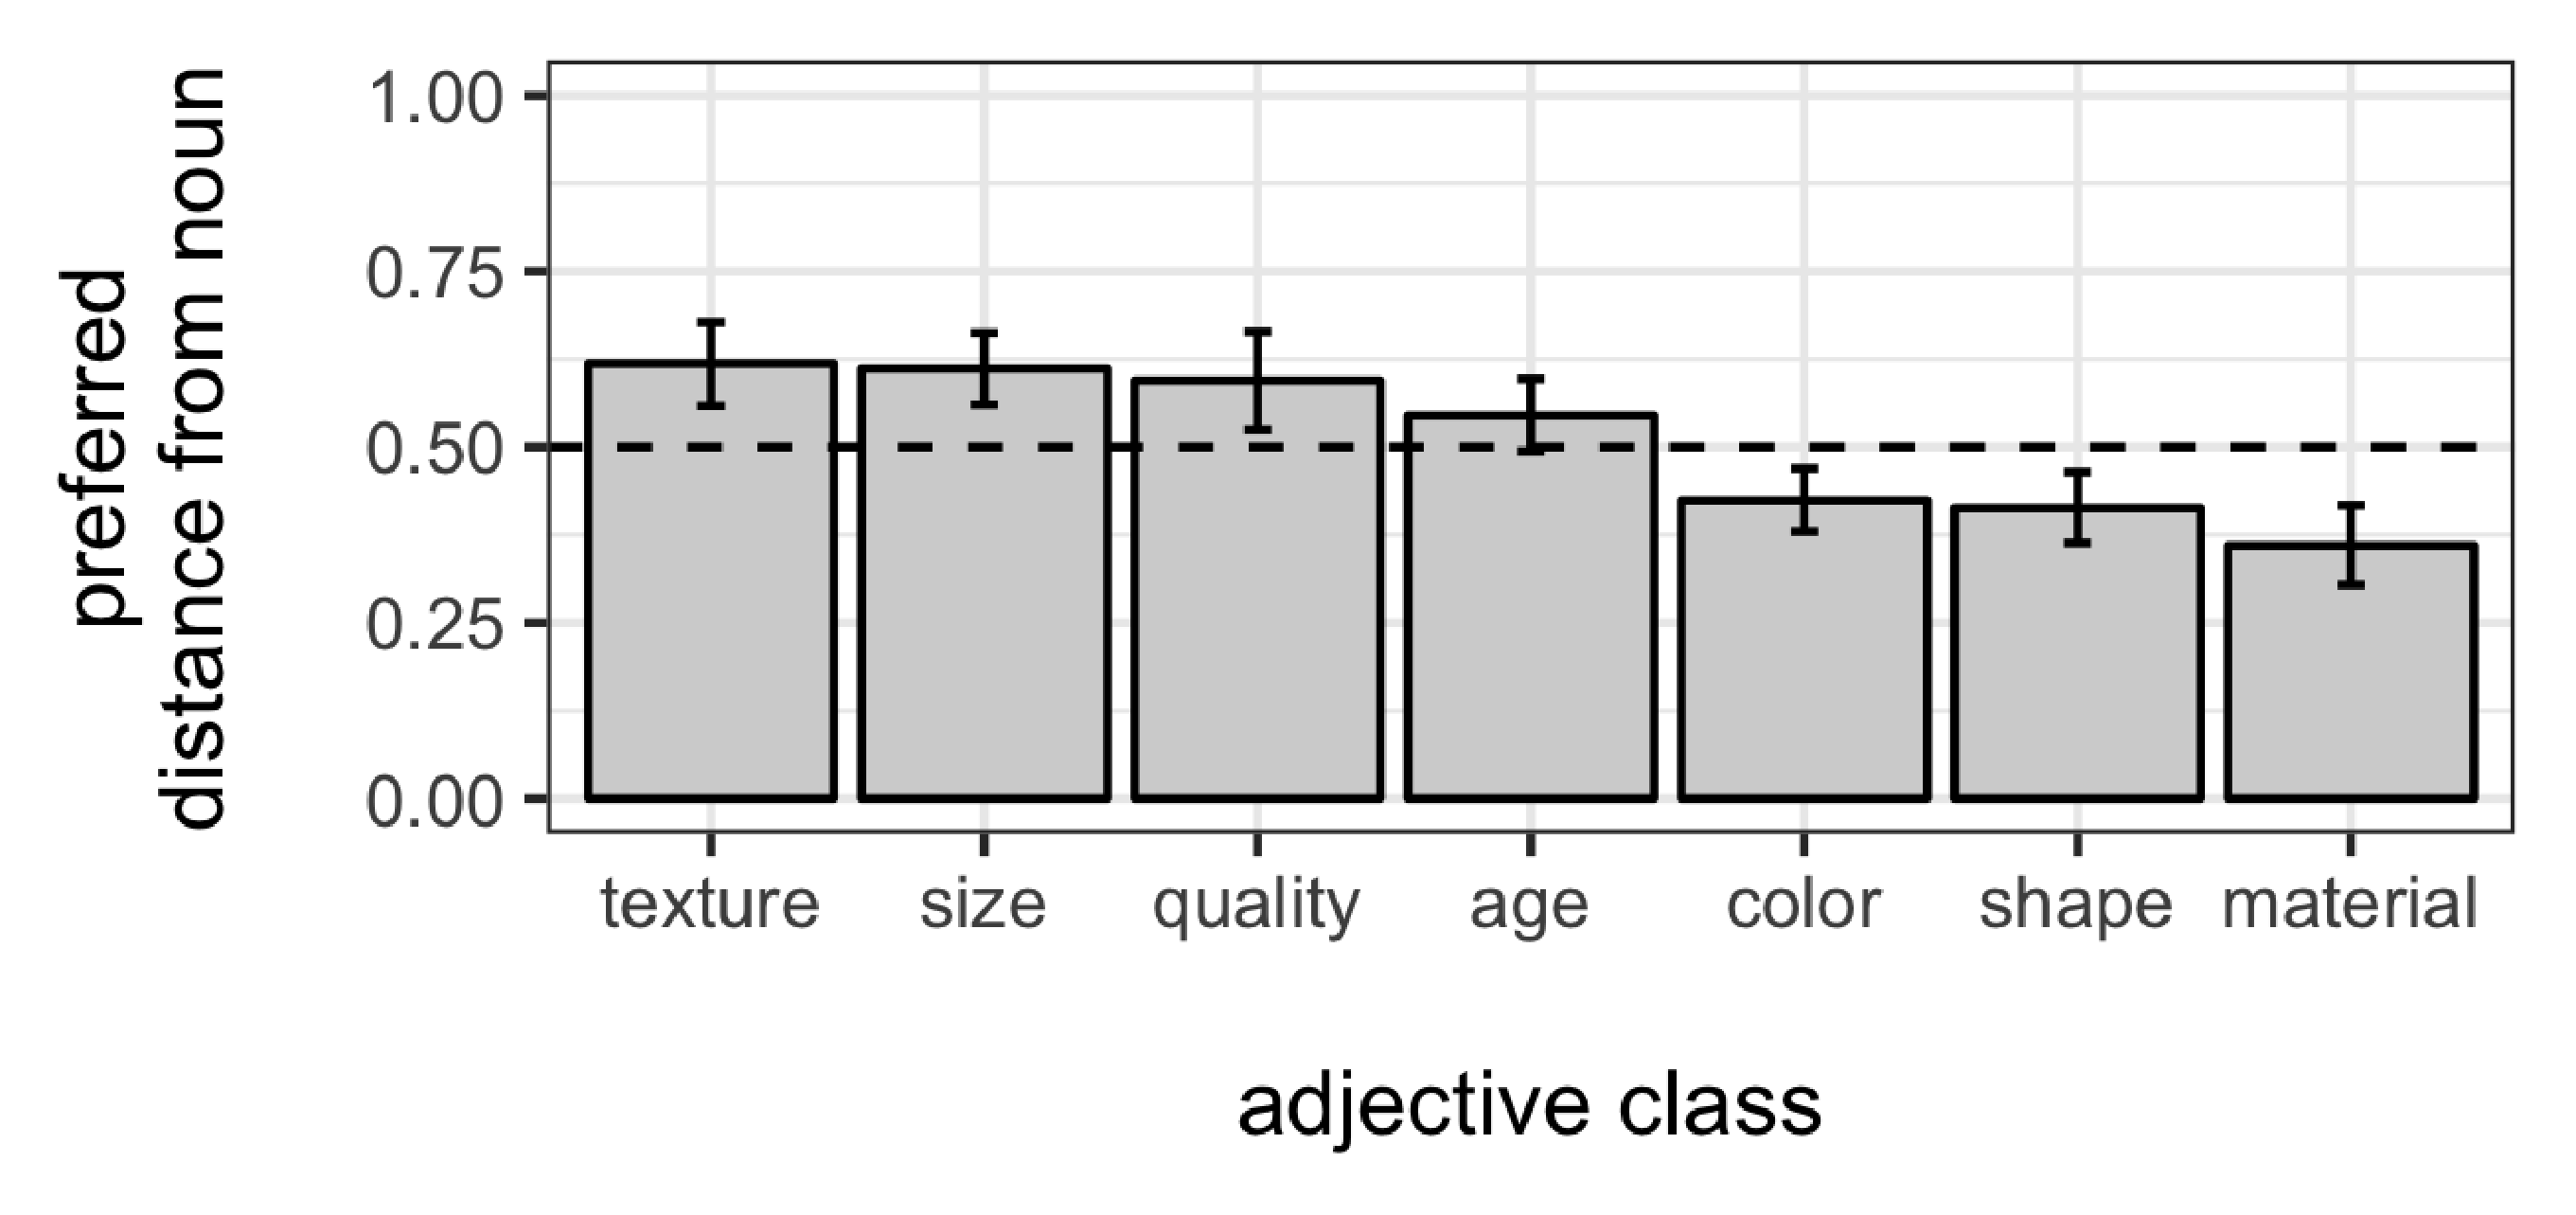
\includegraphics[height=2in]{LSA-class-distance.eps}
	\caption{Naturalness ratings from Experiment 1 grouped by adjective semantic class. Higher values indicate that a class's adjectives are preferred farther from the modified noun; lower values indicate that a class's adjectives are preferred closer. The dashed line indicates chance level, or the absence of stable preferences. Error bars represent bootstrapped 95\% confidence intervals drawn from 10,000 samples of the data.
	}
	\label{exp1-results}
\end{figure}




\section{Experiment 2: Measuring adjective subjectivity} \label{expt2}

Having observed stable ordering preferences in Tagalog, our next task is to measure adjective subjectivity. To do so, we replicated \emph{Expt. 1: Faultless disagreement validation} from \cite{scontrasetal2017adjectives} using the Tagalog materials from Experiment 1.

\subsection{Participants} 

We recruited 45 participants who did not take part in Experiment 1 through Amazon.com's Mechanical Turk. All participants were compensated for their participation. On the basis of their responses to a post-test questionnaire, we identified 11 Tagalog speakers (8 female, 3 male; mean age: 29); their data were included in the analyses below. Of the 11 Tagalog-speaking participants, ten were born in the Philippines and one was born in the United States. Six currently reside in the Philippines, four in the United States, and one in some other country.

\subsection{Procedure}

\begin{figure}[t]
	\centering
	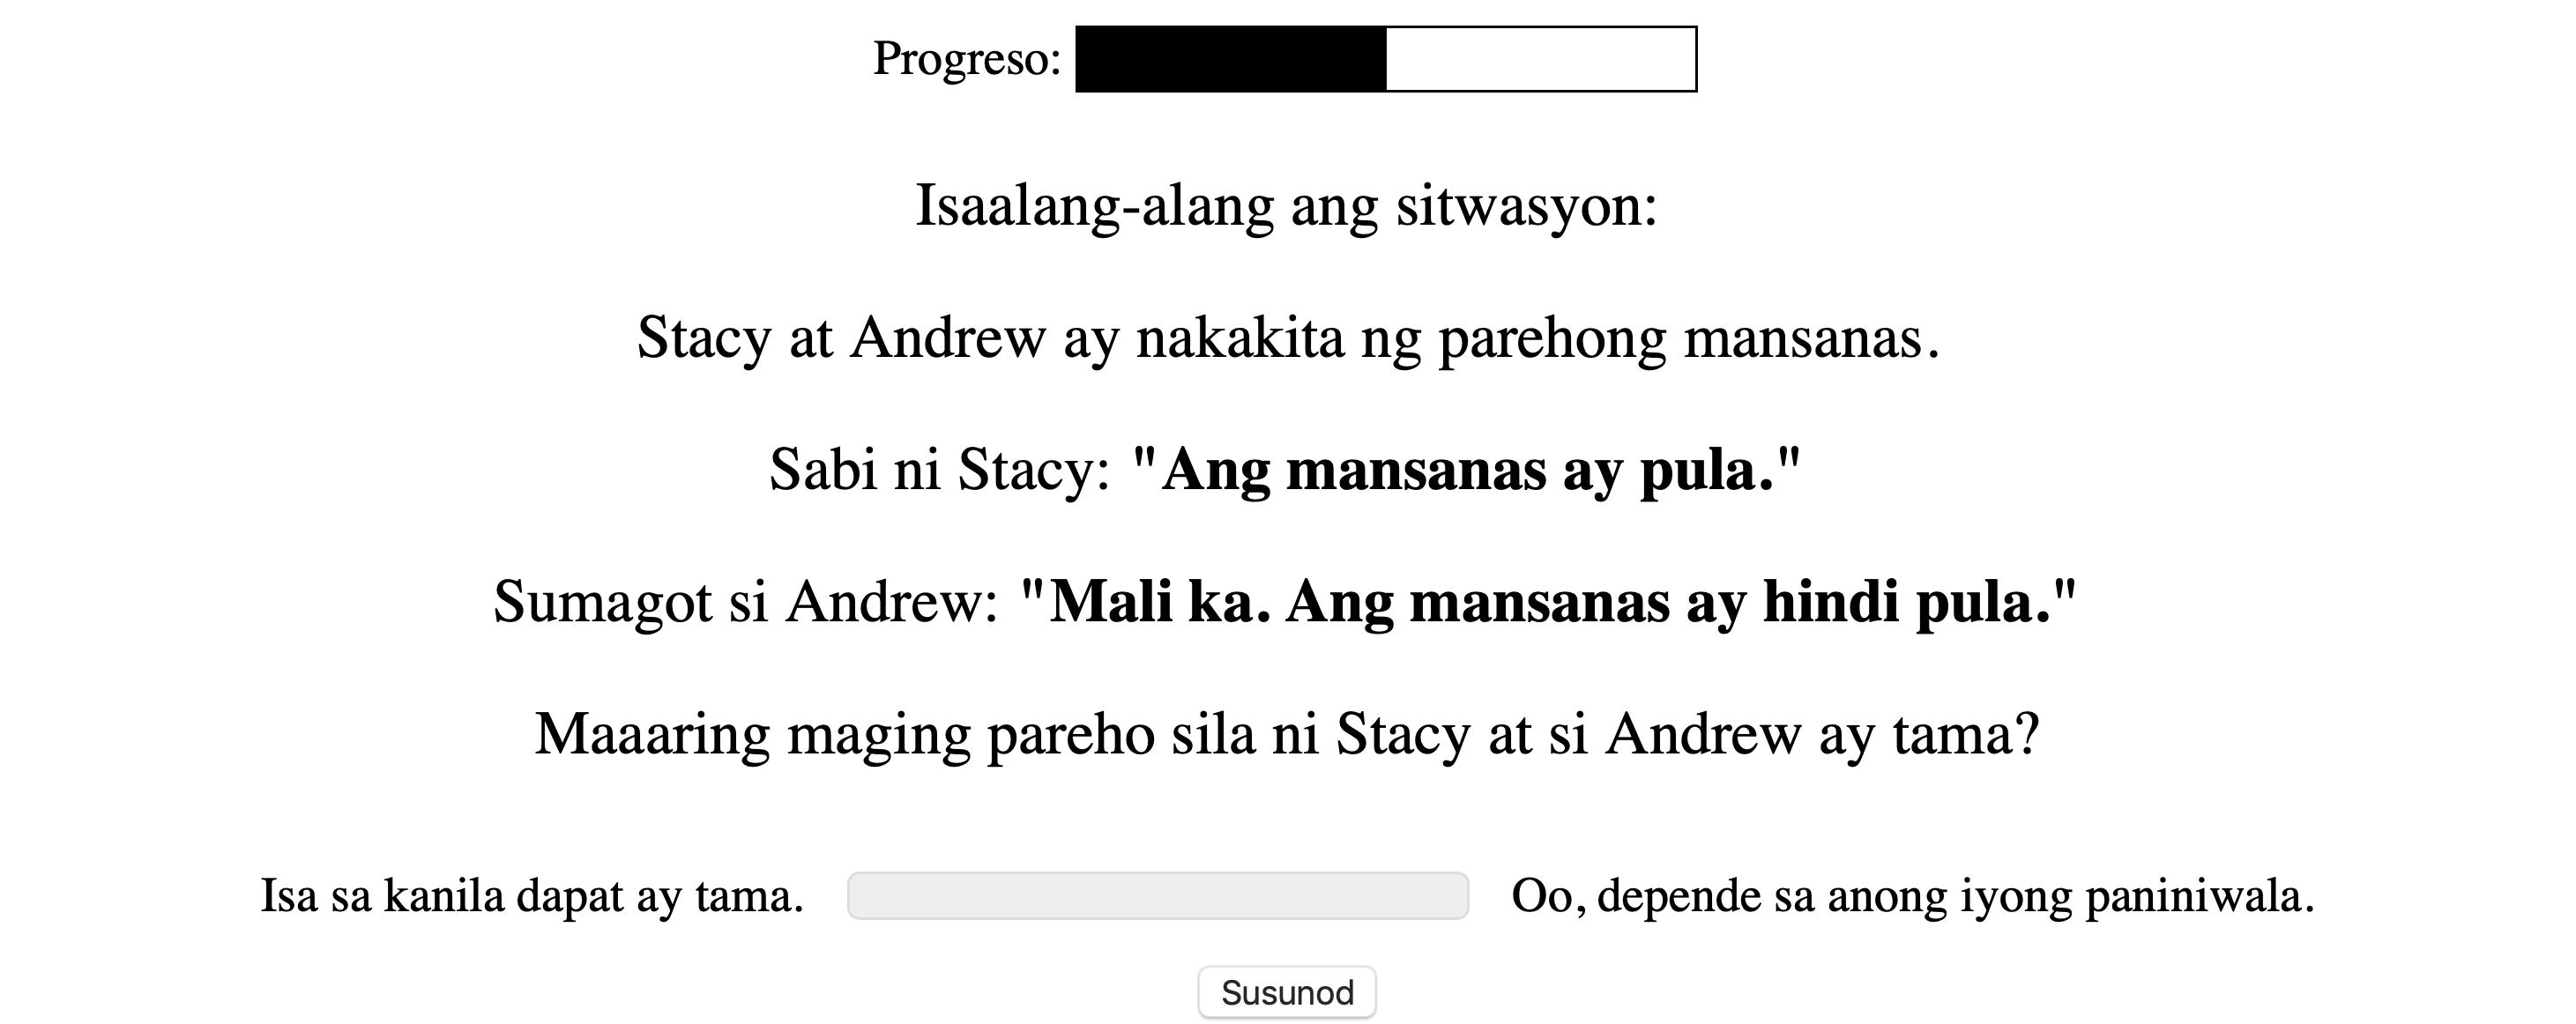
\includegraphics[width=5.9in]{exp2-trial.eps}
	\caption{Sample trial from Experiment 2. Participants rated the possibility for two speakers to faultlessly disagree about a property ascription.
	}
	\label{exp2-trial}
\end{figure}

Participants encountered a series of dialogues in which two speakers disagreed about a property ascription for some object. For example, the two speakers might observe an apple. One speaker would assert that the apple is red, and the other would counter by saying that the apple is not red. Participants judged whether both speakers could be right while disagreeing, or whether one speaker must be wrong. Judgments were provided by adjusting a slider with endpoints labeled `only one can be right' (coded as 0) and `yes, it depends on what you believe' (coded as 1). Figure \ref{exp2-trial} presents an example trial from the experiment.

Participants completed a series of 26 trials in random order, one for each of the adjectives in Table \ref{tagalog-materials}; on each trial, the noun was chosen at random from the list in Table \ref{tagalog-materials}.

\subsection{Results}

We computed a mean faultless disagreement score for each adjective by averaging scores across participants. Figure \ref{exp2-results} plots these faultless disagreement scores grouped by adjective class. We will use the faultless disagreement scores for the individual adjectives in the next section, where we test whether subjectivity predicts ordering preferences in Tagalog.

\begin{figure}[t]
	\centering
	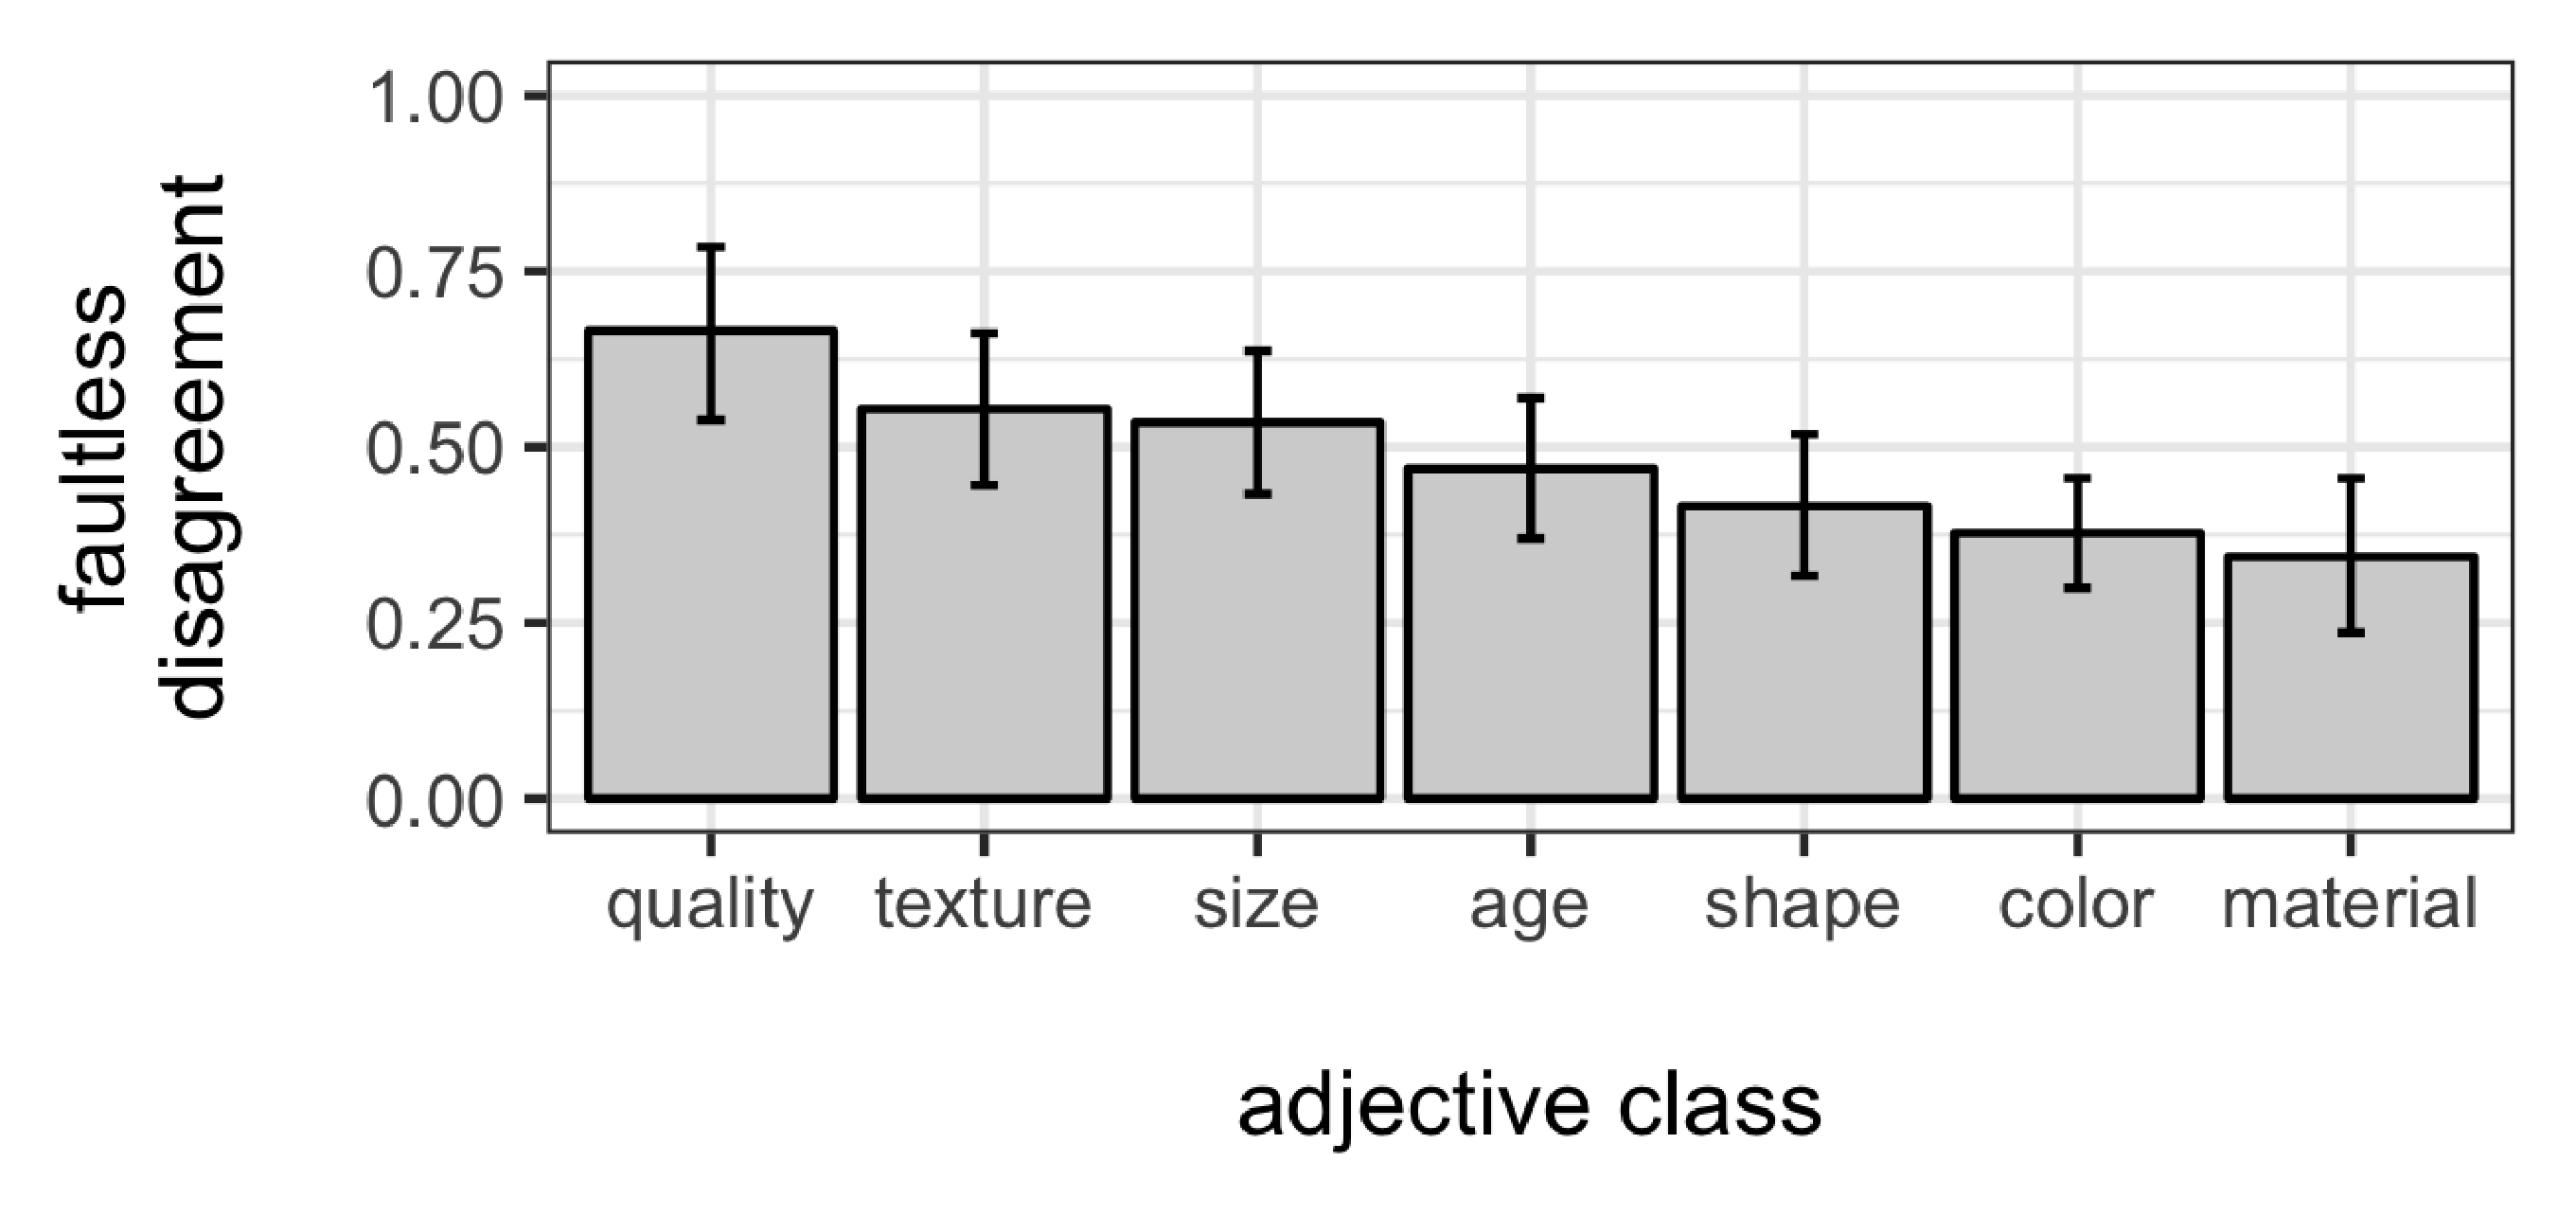
\includegraphics[height=2in]{class_faultless.eps}
	\caption{Faultless disagreement scores from Experiment 2 grouped by adjective semantic class. Higher values indicate that a class's adjectives are perceived as more subjective. Error bars represent bootstrapped 95\% confidence intervals drawn from 10,000 samples of the data.
	}
	\label{exp2-results}
\end{figure}


\section{Comparing ordering preferences with subjectivity} \label{comparison}

With estimates of the Tagalog ordering preferences and adjective subjectivity, our final task is to compare the two measures to determine the extent to which subjectivity predicts Tagalog ordering preferences. Figure \ref{subj-comparison} plots the preferred-distance measures for each of the 26 adjectives against their faultless disagreement (i.e., subjectivity) scores. Adjective subjectivity accounts for 54\% of the variance in the ordering-preference data ($r^2$ = 0.54, 95\% CI = [0.22, 0.74]). In other words, subjectivity does indeed predict adjective ordering preferences in Tagalog.


\begin{figure}[t]
	\centering
	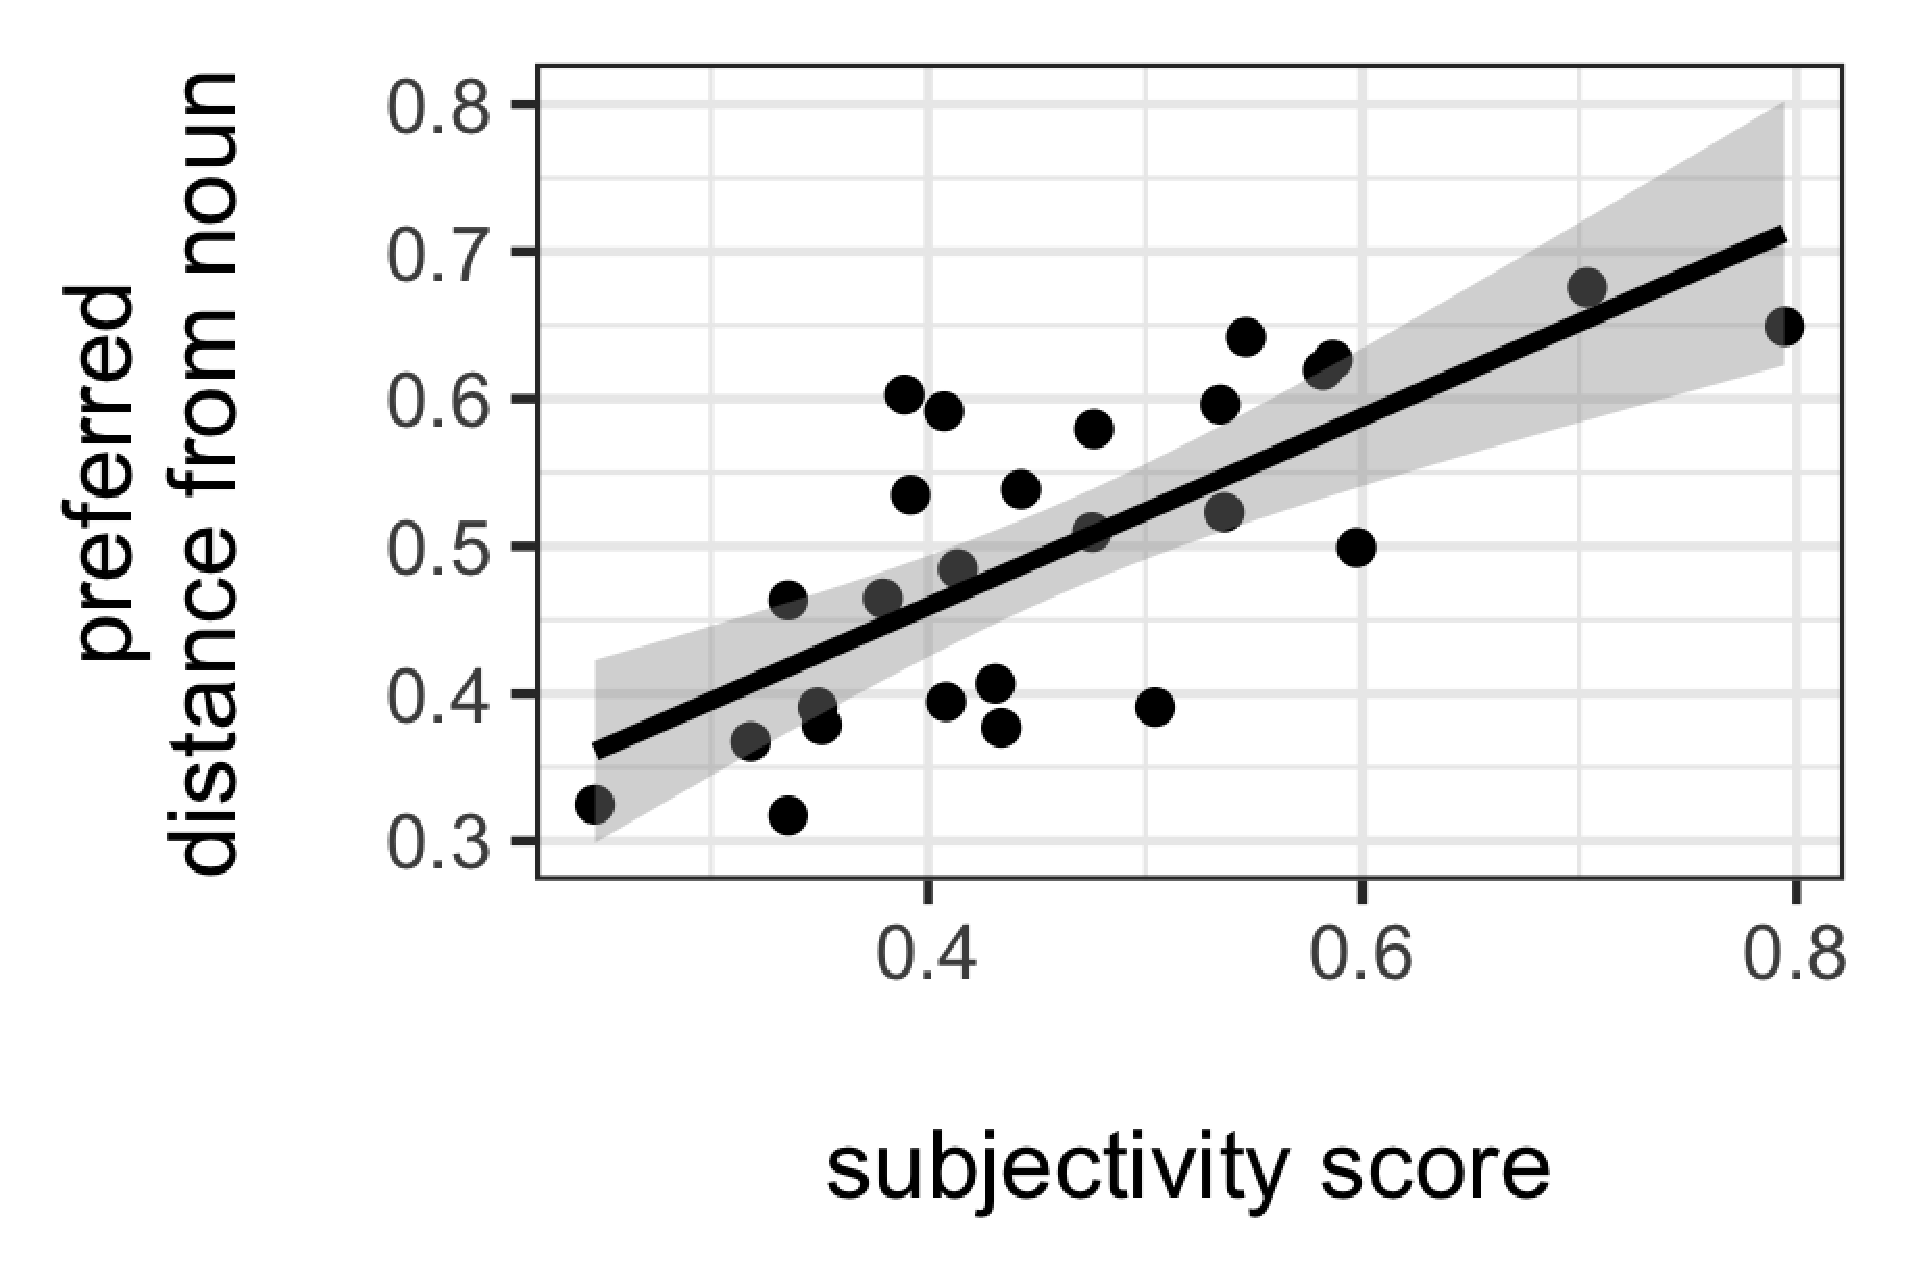
\includegraphics[height=2in]{LSA-naturalness-subjectivity.eps}
	\caption{Ordering preferences (obtained in Experiment 1) plotted against subjectivity scores (obtained in Experiment 2) for each of the 26 adjectives tested. %Subjectivity accounts for 54\% of the variance in the ordering preferences ($r^2$ = 0.54, 95\% CI = [0.22, 0.74]).
	}
	\label{subj-comparison}
\end{figure}


\section{General discussion} \label{discussion}

We have found strong evidence in support of subjectivity-based adjective ordering preferences in Tagalog. Despite the obligatory presence of \textsc{linker} in Tagalog modification structures, the results of Experiment 1 demonstrate that speakers do have stable ordering preferences; these preferences determine the relative order of adjectives in multi-adjective strings. After measuring adjective subjectivity with the faultless disagreement task in Experiment 2, we found that subjectivity predicts the Tagalog preferences, as it does in English. 

Although both Tagalog and English evidence subjectivity-based ordering preferences, there is a salient difference between the results from the two languages: \cite{scontrasetal2017adjectives} found subjectivity to be a much stronger predictor of the English ordering preferences. Using English translations of the materials tested in the current study, the authors observed that subjectivity accounted for between 85\% and 88\% of the variance in the ordering preferences they measured. By contrast, we have found that subjectivity accounts for 54\% of the Tagalog variance---a marked departure from the English baseline.

One might wonder whether the difference we observe between English and Tagalog could be due to imprecise (or impossible) translations. There were eight adjectives in our study that were not translation equivalents with the original English materials (cf.~Table \ref{tagalog-materials}). Perhaps these eight adjectives---nearly a third of the adjectives we tested---led to the poorer performance of subjectivity relative to the English baseline. While we cannot rule out this possibility, we do consider it unlikely that the specific adjectives tested were the sole source of the lower correlation we observe in Tagalog. Rather, there is likely an additional source: the quantity and quality of our Tagalog-speaking participants.

When using Mechanical Turk to collect behavioral data, native speakers of English are ubiquitous among the participant pool; native speakers of Tagalog are not. This fact is reflected in the numbers of participants run in the current study vs.~those run in the studies by \cite{scontrasetal2017adjectives}. We used data from 24 Tagalog speakers to determine ordering preferences, and 11 Tagalog speakers to measure adjective subjectivity; \citeauthor{scontrasetal2017adjectives} had double the number of English speakers for their results. This asymmetry in the number of participants could have introduced more variance in the Tagalog results, such that subjectivity was less capable of explaining it.

Another worry that separates our participants from those in the English study concerns their status as monolingual native speakers. Most speakers of Tagalog are bilingual, and in many cases that bilingualism is imbalanced in favor of a language other than Tagalog. For speakers residing in the Philippines, it is common for Tagalog to be a second language, after one of the many Filipino dialects. And given that the majority of our participants now reside in the United States, we face the possibility that some are English-dominant heritage speakers of Tagalog (for reviews of heritage speakers and the properties of heritage langauges, see \citealp{benmamounetal2013,scontrasetal2015frontiers,montrul2016,polinsky2018book}). Both situations are likely to lead to increased noise in the Tagalog intuitions we measured---noise that would decrease the strength of the correlation between ordering preferences and subjectivity.

Even with these considerations, we still find subjectivity to be a robust predictor of adjective ordering preferences in Tagalog, lending support to the universal nature of the proposed explanations discussed in Section \ref{background}: pressures toward successful communication should apply universally, such that we find subjectivity-based ordering preferences. Both the incremental-processing story of \cite{hahnetal2018} and the hierarchical-composition story of \cite{simonic2018} and \cite{scontrasetalSPadjectives} predict that ordering adjectives in Tagalog according to decreasing subjectivity would maximize communicative success, even in the presence of \textsc{linker}.\\[15pt]

% ---an element some have argued carries a semantics similar to conjunction---

% A major influence for this study was the work completed by Scontras, Degen and Goodman (2017). Unlike the English baseline, Tagalog adjective ordering preferences had yet to be studied. It was unknown whether or not the mechanisms of English generalized to other languages, let alone Austronesian languages such as Tagalog. Tagalog holds a different format from English when forming modification structures, utilizing \textsc{linker}s (i.e. -ng, na) which might act similarly to conjunctions when forming multi-adjective strings. The English study was thus replicated in Tagalog to determine whether there are ordering preferences in the presence of \textsc{linker}, as well as to see if subjectivity was significant in predicting ordering preferences cross-linguistically. 

% As compared to the Scontras, Degen, and Goodman (2017) experiment, although the effect might be smaller (r2 = 0.54 vs. r2 = 0.85), Tagalog does seem to follow the same trend as English, placing less subjective adjectives closer to the modified noun. Despite the addition of  a \textsc{linker}, which is semantically similar to conjunction, subjectivity still predicts adjective ordering preferences in Tagalog. As seen in Figure 6, greater values signal that an adjective is more subjective, and lower values signal that they are less subjective. Classes such as quality, texture, and size are seen as more subjective whereas color and material are seen as less subjective. As subjectivity scores increase, these adjectives are preferred farther from the noun, with lower scores indicating that the adjectives are preferred closer to the noun. Examples of more subjective adjectives are Maganda (nice) and Malaki (big), and examples of the less subjective adjectives are Aluminyo (aluminum) and Pula (red). 

% With an r2 = 0.54, the remaining 0.46 of variance can be due to internal factors within the study, or it could represent noise in the data. One potential difference with the English study stems from the use of imprecise translations or alternative lexical terms. The words that were changed can be identified in Table 1 as those bolded and italicized. These words were chosen based on their similarity to the original adjectives and nouns based off of semantic class. For example, adjectives changed under the color class were replaced with another color word, dimension class adjectives with another dimension class adjective, etc. Similarly for nouns, the words that were chosen in replacement were changed with another noun that also could be classified as either food or furniture.  

% As seen in Figure 6, there are outliers in the data such as Bago (new), Maikli (short), Sariwa (fresh), Maganda (nice), Cuadrado (square), Kahoy (wooden), and Berde (green). Bago (new) and Maikli (short) were preferred farther away from the noun than one would expect based off of subjectivity scores, with the rest preferred closer to the noun. This might be due to instances in which the words were used; some participants might never have strung certain words together and had to settle with their best guess, or might have been unfamiliar with how to describe the object with the given words. Furthermore, ``cuadrado'' (square) is a longer word and it is preferred closer to the noun than we would expect on the basis of subjectivity. Similar word length effects have been observed in English (Wulff, 2003; Scontras, Degen and Goodman, 2017). 

% Noise might have been introduced by the participants tested as well. The current study had fewer participants surveyed than in the original English experiment. The Scontras, Degen, and Goodman (2017) study tested 90 subjects total, whereas the current Tagalog replication tested 35 subjects. There is a clear gap in participation between the two experiments. Among the participants tested, many were bilinguals (a speaker who knows fluently both Tagalog and another language), and some were likely heritage speakers. Heritage speakers are ``unbalanced bilinguals, simultaneous or sequential, who shifted early in childhood from one language (their heritage language) to their dominant language (the language of their speech community)'' (Scontras, Fuchs and Polinsky 2015). For example, a speaker shifting from Tagalog at a young age to English would be an English-dominant heritage speaker of Tagalog. This alone could have also created noise in the data and should be controlled for in future research. 

% This study could be improved by including a broader set of words in order to account for possible outliers and difficulties in translation, as well as testing more subjects in order to normalize the data. Furthermore, future directions could study explicitly bilinguals or heritage speakers in order to explore potential effects of speaker profile on ordering preferences. Other directions might investigate ordering preferences in Tagalog speaking children to see when in language development these preferences arise. 

% Though it has been accepted that subjectivity is a major predictor in adjective ordering preferences--now understood to influence cross-linguistically, as evidenced by the current results--it is still unknown what cognitive mechanism forms this subjectivity. In time, future work might delve into the cognitive mechanisms that cause these preferences in language, as a means of better understanding the human mind.
 
% 
%\section{Citations and references} Use author-date notation for in-text citations, for example: ... as noted recently by Jameson (2012) and Mateus (2014), drawing on insights from various other researchers (e.g., Nelson 1986:223-28, Martin 2003, Wellington \& Johnson 2016), there have been numerous technological advances in the procedures used to publish research articles online. Include URLs or DOIs with active hyperlinks in citations. The \textit{Semantics and Pragmatics} stylesheet \href{https://raw.githubusercontent.com/semprag/tex/master/sp.bst}{sp.bst} meets the LSA formatting requirements for the list of references, and so may be used. See \href{http://info.semprag.org}{info.semprag.org}. 
 
% ------------ references --------------------------------------------------------------------------------------
\setlength{\bibsep}{0pt plus 0.3ex}
\setlength{\bibhang}{0.3in}			% hanging indent for references must be 0.3in
\titleformat{\section}{\normalfont\bfseries}{\thesection}{.5em}{}		% references section not supposed to be followed by a period


\bibliographystyle{sp.bst}		% S\&P bibliography style
%S\&P, an LSA publication, meets the LSA guidelines. 
%See: http://info.semprag.org 
%and get the bst at: https://raw.githubusercontent.com/semprag/tex/master/sp.bst 
%If using the sp.bst, the following command turns your DOIs into links
\newcommand{\doi}[1]{\href{http://dx.doi.org/#1}{http://dx.doi.org/#1}}	%modified from sp.cls
\bibliography{greg}			% your bib file

\end{document}
 
 
 
 